Um die Funktionsweise des Newsboards wird zuerst das zugrunde liegende Konzept erläutert.
Dazu gehören neben Architekturentscheidungen auch das Datenmodell und die Schnittstelle
zur Kommunikation mit den externen Modulen.

\subsection{Architektur}
Der erste richtungweisende Punkt für des Konzepts ist die Architektur des Newsboards.
Da eine Webseite zum Einsehen der bewerteten Nachrichten eine der Voraussetzungen ist,
bietet sich eine klassische Client-Server-Architektur an.
Dabei treten neben den Webbrowsern des Benutzer auch die Crawler-
und Bewertungsmodule als Clients auf.

Um die Komplexität des Newsboads möglichst gering zu halten, sollte die Kommunikation
mit den Modulen ebenfalls über HTTP stattfinden. Das bringt den Vorteil mit sich,
dass es für viele Programmiersprachen bereits gute Client-Bibliotheken gibt
und sich so keine unnötigen Einschränkungen ergeben.

\subsection{Datenmodell}
Bei der Analyse der zu persistierenden Daten wurde ebenfalls darauf geachtet, ein
sowohl möglichst einfaches, aber auch flexibles Datenmodell zu entwickeln. Zu Projektbeginn wurden verschiedene klassisch-relationale Datenbanksysteme mit diversen 
NoSQL-Techniken verglichen. So schien es durchaus plausibel, eine der verschiedenen
NoSQL-Varianten einsetzen zu können, um Daten schemafrei und somit sehr flexibel 
ablegen zu können. Bei der Recherche dieser Systeme konnte jedoch keine NoSQL-
Technologie überzeugend Mehrwert liefern. Deshalb setzt das Newsboard in der jetzigen Form 
auf ein relationales Modell zur Persistenz, da diese Systeme mehr
verbreitet, ausgereift und dokumentiert sind.

Das folgende Entity-Relationship-Diagramm gibt eine Übersicht über die im Newsboard
vorhandenen Entitäten und ihre Attributen:

\begin{figure}[h]
	\centering 
	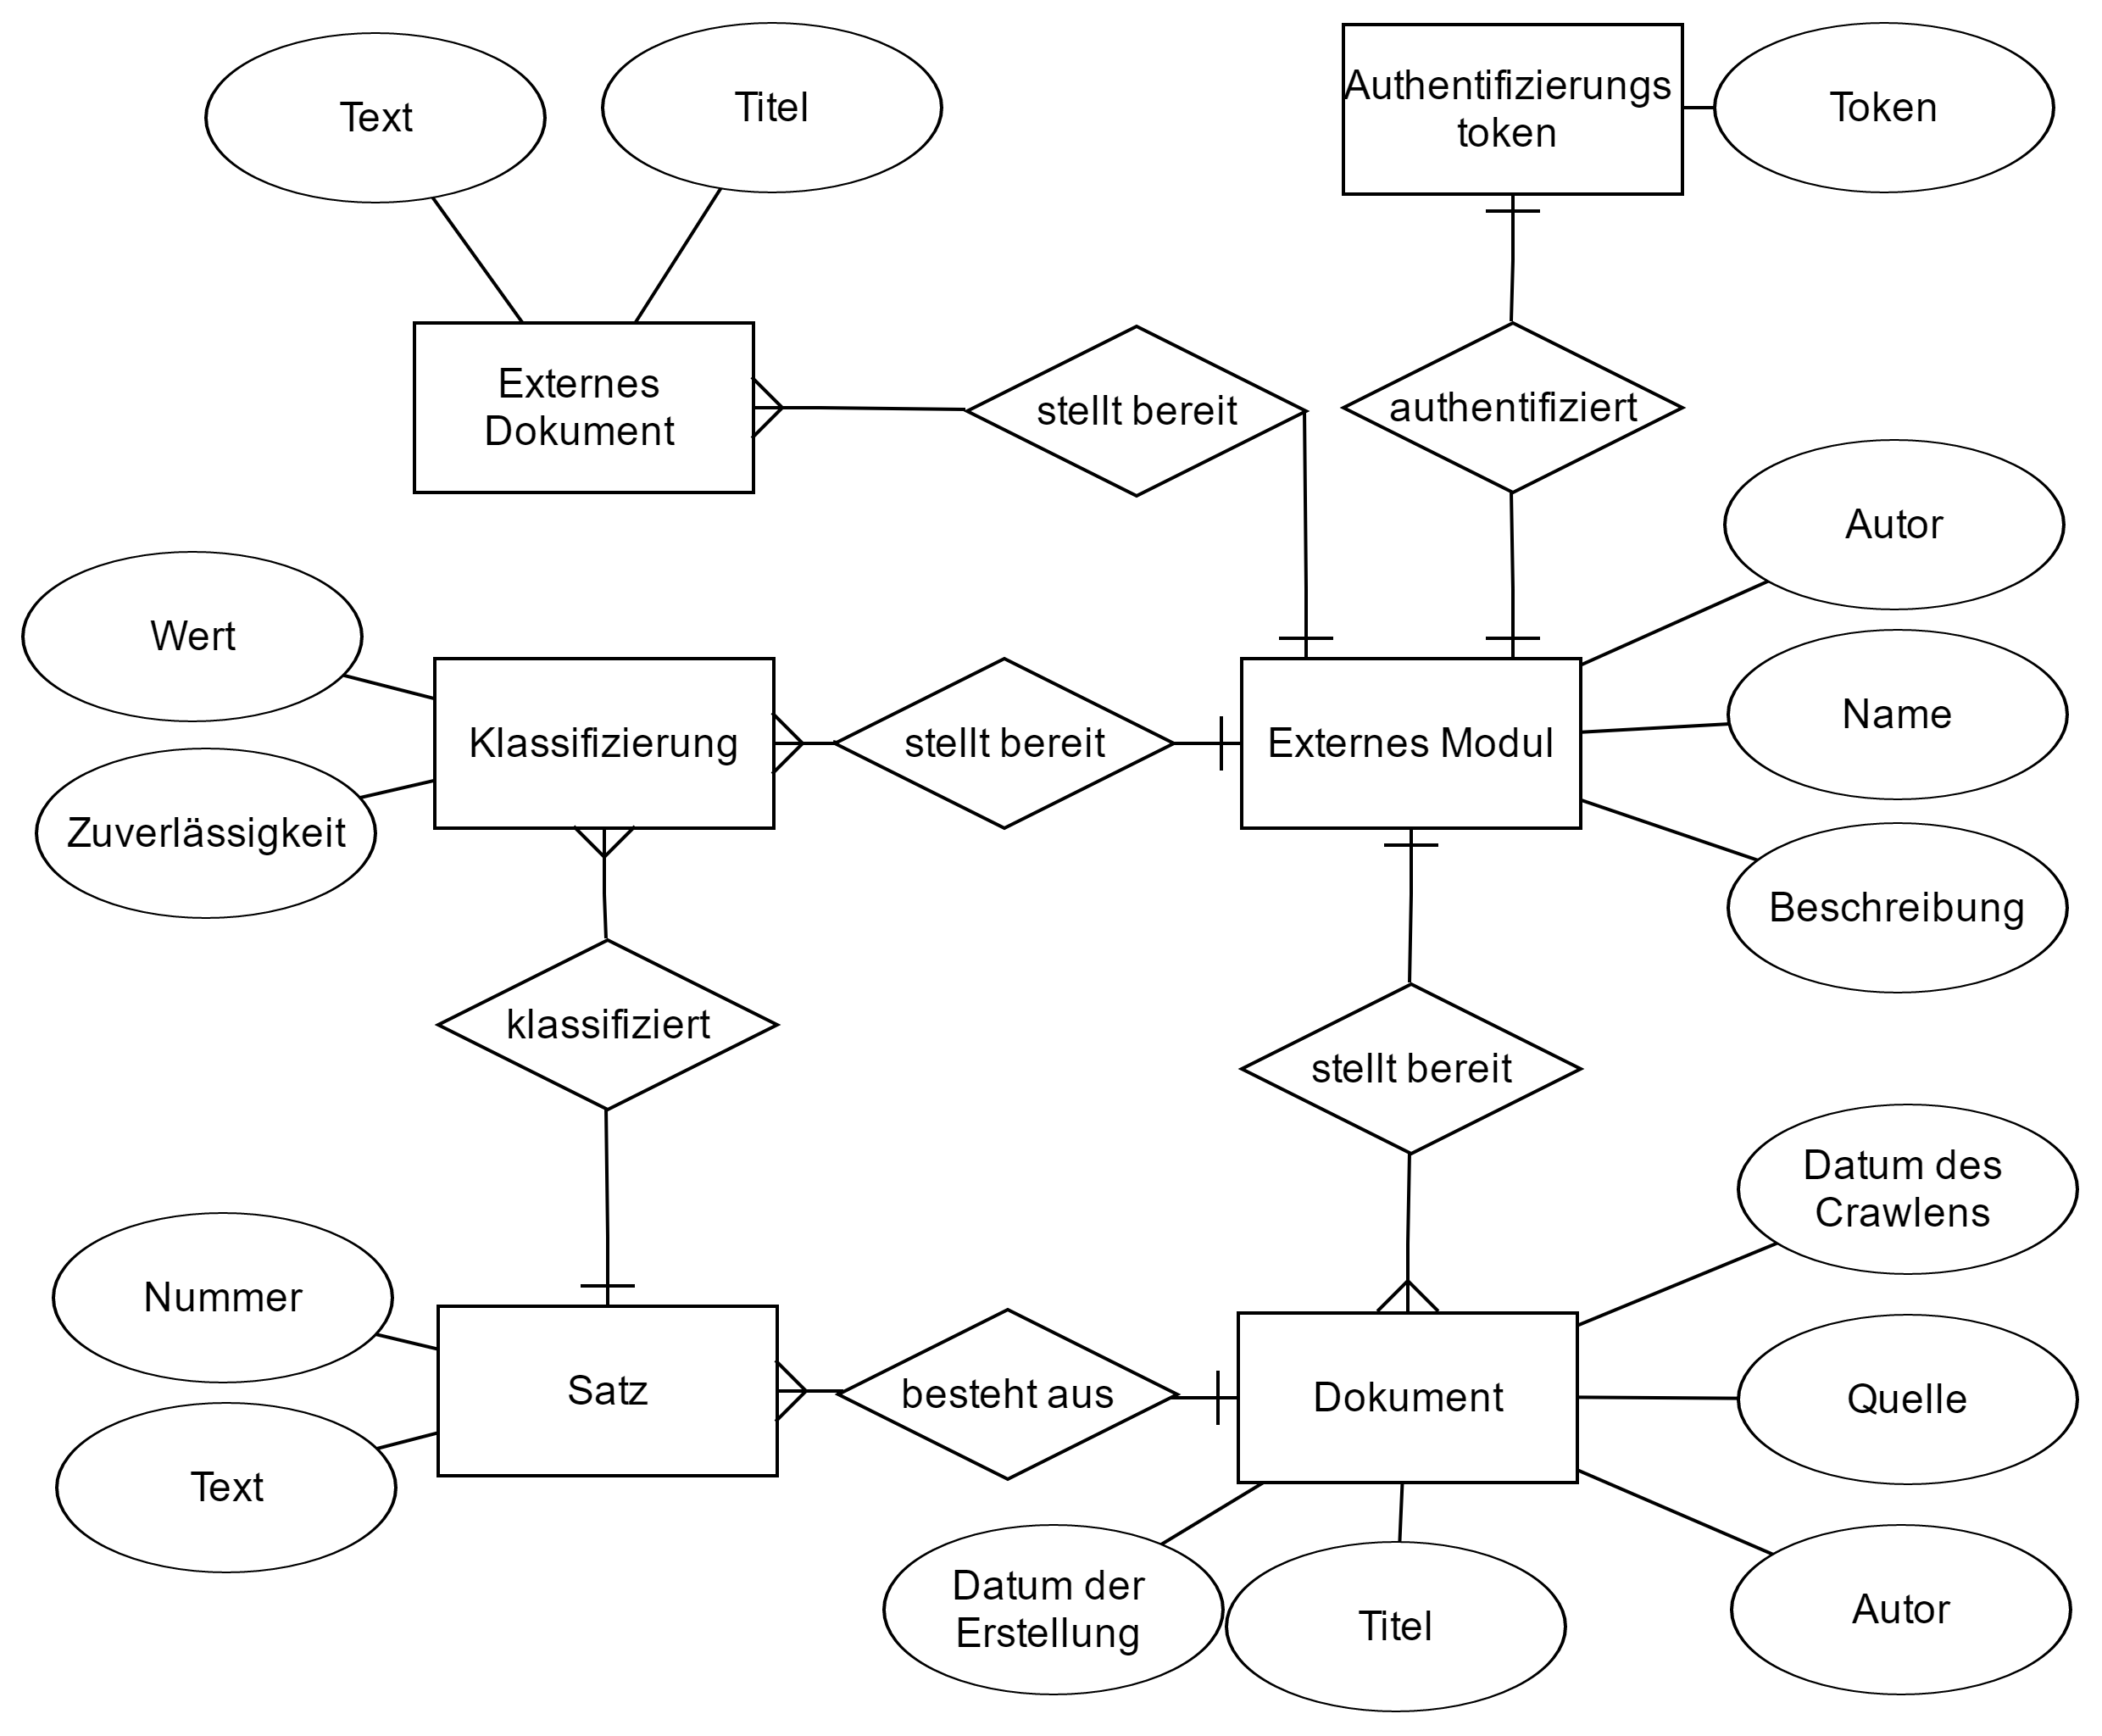
\includegraphics[scale=0.175]{content/erd.png}
	\label{erd}
	\caption{ERD des Newsboards}
\end{figure}

Wie aus dem ERD ersichtlich, besteht das Newsboard aus diesen nun näher beschriebenen 
Entitäten:
\begin{itemize}
	\item \textbf{Externe Module}\\
	Die externen Systeme, die Daten für das Newsboard hochladen, werden in dieser Tabelle
	gespeichert. Von Interesse sind Informationen über den Autor des Moduls,
	den Namen sowie eine kurze Beschreibung.
	\item \textbf{Authentifizierungstoken}\\
	Authentifizierungstokens dienen zur Bestätigung der Identität von externen Modulen.
	Nur Module, die über ein gültiges Authentifizierungstoken verfügen, dürfen in der Lage
	sein, Daten für das Newsboard hochzuladen. Ein Token besteht aus einer zufälligen
	Zeichenkette.
	\item \textbf{Externe Dokumente}\\
	Dokumente oder Nachrichten, die nicht klassifiziert, dem Gesamtsystem aber dennoch zur
	Verfügung stehen sollen, werden als externe Dokumente gespeichert. Der Inhalt dieser
	Dokumente wird als Plaintext abgelegt. Auch der Titel des Dokumentes ist von Interesse.
	\item \textbf{Dokumente}\\
	Nachrichten und Texte, die im Newsboard dargestellt werden sollen oder zur
	Klassifizierung bereitstehen, werden als Dokumente im System abgelegt. Der eigentliche
	Text wird in Sätze aufgeteilt abgelegt, über die Dokumente selbst werden aber einige
	Metainformationen gespeichert. Hierzu zählen zum Beispiel das Datum der Erstellung und
	des Crawlens, der Autor sowie der Titel und die Quelle des Dokumentes
	\item \textbf{Sätze}\\
	Die eigentlichen Sätze, die in einem Dokument geschrieben sind, werden separat 
	gespeichert. Sie sind es auch, die zur Klassifizierung von externen Modulen 
	bereitstehen. Um ein Dokument wieder korrekt zusammenzusetzen, wird zu dem die 
	Position eines jeden Satzes im Dokument als Nummer gespeichert.
	\item \textbf{Klassifizierungen}\\
	Die Klassifizierungen der Sätze werden in dieser Tabelle gespeichert. Neben den 
	Informationen, zu welchem Satz eine Klassifizierung gehört, muss zudem das 
	klassifizierende Modul abgelegt werden. Eine Klassifizierung selbst besteht aus zwei 
	Werten: einem für den errechneten Wert und einem für die Zuversichtlichkeit des Moduls,
	wie genau die Klassifizierung ist. 
\end{itemize}

\subsection{Schnittstelle}
Die Hauptziele bei der Konzeption der Schnittstelle waren zum einen eine möglichst
einfache Verwendung, sowie eine verlässliche Validierung der Übertragenen Daten.
Da die Schnittstelle auf HTTP aufbaut, bietet es sich an, REST zu verwenden.

Als Datenformat für die Schnittstelle bieten sich sowohl JSON, als auch XML an.
Da XML im Gegensatz zu JSON allerdings eine verlässliche Möglichkeit zur Validierung
und Dokumentation durch ein Schema besitzt, ist es in diesem Fall die bessere Wahl.
Der geringfügig höhere Speicherverbrauch, sowie die derzeit geringe Popularität
von XML sollen hier keine Rolle spielen.

Bei der Konzeption der verwendeten REST-Ressourcen, sowie deren akzeptierten Methoden
bestehen ebenfalls zwei mögliche Szenarien. Das erste ist die Abbildung sämtlicher
Datentypen des Datenmodells und das Erlauben aller CRUD-Operationen.
Das zweite Szenario ist es, ausschließlich einige wenige Ressourcen zur Verfügung
zu stellen, welche die geplanten Anwendungsfälle abbilden.

Letzteres verlangt komplexere Daten, die von der Schnittstelle verarbeitet werden müssen,
andernfalls läge diese Komplexität jeweils in den einzelnen Clients und müsste
mehrfach konzeptioniert und umgesetzt werden. Das führt letztendlich zu mehr
unnützer Arbeit und gleichzeitig zur mehr potentiellen Fehlerquellen.
Da für diese Schnittstelle potentiell regelmäßig neue Clients entwickelt werden sollen,
ist die zweite Variante als deutlich zweckmäßiger, sowie allgemein eleganter anzusehen.

Die sich aus den Anwendungsfällen und konzeptionellen Vorüberlegungen resultierenden
Aktionen, welche durch die REST-Schnittstelle ermöglicht werden, lauten wie folgt:
\begin{itemize}
	\item Einfügen neuer Dokumente
	\item Lesen von Dokumenten
	\item Einfügen neuer Klassifizierungen für Dokumente
\end{itemize}
